\section{Realimentación lineal de estados}

Se solicita realizar una realimentación lineal de estados tal que la ganancia en continua del sistema sea unitaria y e sobrepico porcentual (OS) sea inferior a un 25\%.

Con tal de realizar la realimentación se verifica que el sistema sea totalmente controlable. Para ello se emplea la matrix controlabilidad:

\begin{equation}
    C_m = \begin{bmatrix} 
        B & AB 
    \end{bmatrix} = 
    \begin{bmatrix}
        0 & G_0 \\ G_0 & 0
    \end{bmatrix}
\end{equation}

\noindent donde se observa que la matrix en cuestión es de rango completo ($det(C_m) = -G_0^2 \neq 0$), por lo que el sistema es totalmente controlable. 

Una vez que se confirma la controlabilidad del sistema es posible continuar con la ecuación característica del sistema realimentado:

\begin{equation}
    |s\mathbb{I} - A + B \cdot k| = s^2 + s \cdot G_0 \cdot k_2 + G_0 \cdot k_1
\end{equation}

\noindent donde, por un lado, resulta evidente la condición para que el sistema resultante disponga de ganancia unitaria en continua:

\begin{equation}
    k_1 \cdot G_0 = G_0 \Longrightarrow \boxed{k_1 = 1}
\end{equation}

\noindent Por otro lado, con tal de obtener $k_2$ hemos de escribir la ecuación característica de un segundo orden:

\begin{align*}
    s^2 + s \cdot 2\xi \omega_n + {\omega_n}^2
\end{align*}


\noindent de este modo:

\begin{equation}
    k_2 = \frac{2\xi \sqrt{k_1}}{\sqrt{G_0}}
\end{equation}

\noindent Con tal de alcanzar las especificaciones de sobrepico solicitadas se ha de prestar atención a la relación:

\begin{equation}
    OS = e^{-\frac{\pi \cdot \xi}{\sqrt{1-\xi^2}}}
\end{equation}

\noindent tal que:

\begin{equation}
    \xi = \sqrt{\frac{ln(OS)^2}{\pi^2 + ln(OS)^2}}
\end{equation}

\noindent remplazando:

\begin{equation}
    k_2 = \sqrt{4 \cdot \frac{ln(OS)^2}{\pi^2 + ln(OS)^2} \cdot \frac{k_1}{G_0}} \Longrightarrow \boxed{k_2= 0.05535}
\end{equation}


\noindent De este modo el sistema a implementar corresponde con:

\vspace{1cm}
\begin{figure}[H]
  \centering
  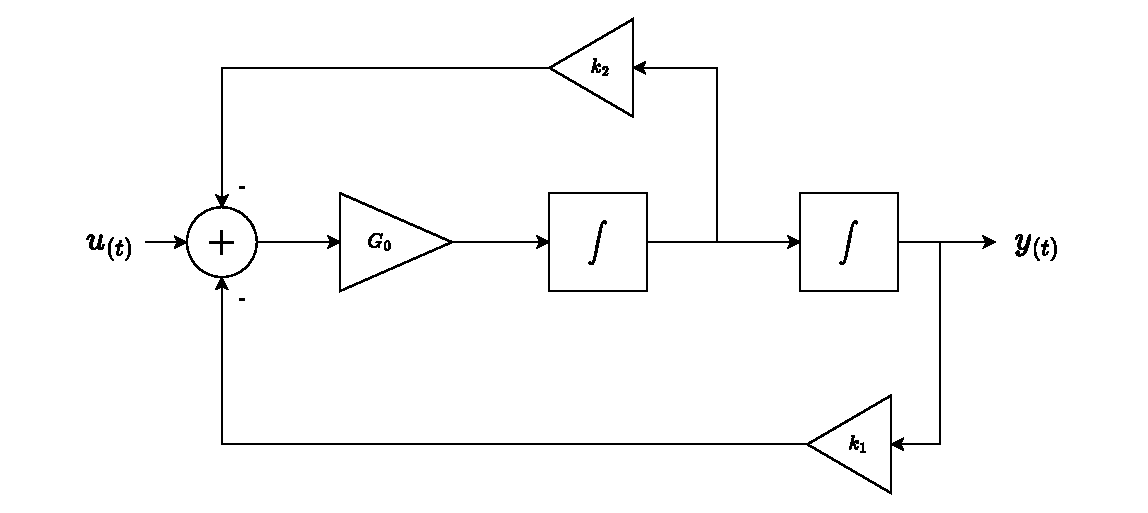
\includegraphics[width = \textwidth]{Imagenes/2_Analisis_lazo_abierto/lazo cerrado.drawio.pdf}
  \caption{Sistema a lazo cerrado | Diagrama en bloques.}
  \label{fig: sistema a lazo cerrado diagrama}
\end{figure}
